% Dokumentenklasse definieren.
\documentclass[
    12pt,
    a4paper,
    doubleside,
    BCOR=10mm,
    parskip=half,
    ngerman
]{scrbook}

% Die Header-Datei enthält alle verwendeten Pakete, sowie 
% Konfigurationen für Farben der Links und die Kopf- und 
% Fußzeilen. 
% Für den Druck kann "header.tex" in "header_print.tex" geändert werden, damit alle Verlinkungen und Markups schwarz bleiben.
\usepackage[utf8]{inputenc}
\usepackage[T1]{fontenc}

% Deutsches Sprachpaket für Babel auswählen
\usepackage[german] {babel}

% Font Änderungen
\usepackage{lmodern}
\usepackage[scaled]{helvet}
\renewcommand\familydefault{\sfdefault} 

% Integration von PDF Seiten. Wird zum Einfügen der eidesstattlichen Erklärung der Thesis verwendet.
\usepackage{pdfpages}

% Lipsum Fließtext generieren mit \lipsum 
\usepackage{lipsum}
\usepackage{cprotect}
\usepackage{csquotes}

% Kopf- und Fußzeilen der Seiten anpassen 
\usepackage{fancyhdr}

% Ersetzt \hline in Tabellen mit \toprule, \midrule und \bottomrule
\usepackage{booktabs}

% Unter anderem für mathematische Formeln
\usepackage{amsmath}

% Enthalten mathematische Symbole
\usepackage{amsfonts}
\usepackage{kpfonts}
\usepackage{amssymb}

% Generiert graphische Elemente, wie beispielsweise Diagramme
\usepackage{tikz}

% Bilder in Latex einbinden mit \includegraphics
\usepackage{graphicx}

% Den Pfad für alle Bilder relativ zur header.tex-Datei setzen.
\graphicspath{ {images/} }

% Tabellen automatisch an die Textbreite anpassen
\usepackage{tabularx}

% Mehrere Reihen in einer Tabelle zusammenschließen
\usepackage{multirow}

% Mehr Farben für LaTeX
\usepackage{xcolor}
\usepackage{color}
\definecolor{dkgreen}{rgb}{0,0.6,0}
\definecolor{dkblue}{rgb}{0,0,0.2}
\definecolor{gray}{rgb}{0.5,0.5,0.5}
\definecolor{mauve}{rgb}{0.58,0,0.82}
\definecolor{darkerred}{rgb}{0.2,0,0}

% Paket, um Links im Dokument zu erzeugen
\PassOptionsToPackage{hyphens}{url}\usepackage{hyperref}

% Farben und Art der Links anpassen
\hypersetup{
    colorlinks = true,
    linkcolor=black,
    filecolor=black,      
    urlcolor=black,
    citecolor=black
}

% Enumerationsliste mit römischen Zeichen
\renewcommand{\theenumi}{\roman{enumi}}
\usepackage{footnote}
\makesavenoteenv{figure}
\usepackage{epigraph}
\usepackage{listings}

% Umlaute in Listings zulassen
\lstset{literate=% Allow for German characters in lstlistings.
{Ö}{{\"O}}1
{Ä}{{\"A}}1
{Ü}{{\"U}}1
{ß}{{\ss}}2
{ü}{{\"u}}1
{ä}{{\"a}}1
{ö}{{\"o}}1
}

% Farben in Lstlistings verwenden
\lstset{frame=tb,
    language=Java,
    aboveskip=3mm,
    belowskip=3mm,
    showstringspaces=false,
    columns=flexible,
    basicstyle={\small\ttfamily},
    numbers=none,
    numberstyle=\tiny\color{black},
    keywordstyle=\color{black},
    commentstyle=\color{black},
    stringstyle=\color{black},
    breaklines=true,
    breakatwhitespace=true,
    tabsize=3
}

% Paket für Akronyme und Glossar
\usepackage[acronym,nonumberlist,order=letter,nopostdot,toc,numberedsection=autolabel,section=chapter]{glossaries}
%,style=super
\renewcommand*{\glspostdescription}{}
\setacronymstyle{long-short}

% Ändern der Farbe für Verlinkungen auf die Akronyme und in das Glossar auf ein dunkles Rot.
\renewcommand*{\glstextformat}[1]{\textcolor{black}{#1}}
\makenoidxglossaries{}

\usepackage[doublespacing]{setspace}
\usepackage{background}
\usepackage{lastpage}

% Mit dem Command \subautor kann jedem einzelnen Kapitel ein einzelner Autor hinzugefügt werden
\newcommand{\subautor}[1]{\begin{flushright}
    {\small\textit{#1}}    
\end{flushright}}

% Notwendig, um die Verlinkung in das Inhaltsverzeichnis über die Fußzeile zu erstellen.
\backgroundsetup{contents={}}

% Normaler Stil für Seiten innerhalb der Arbeit
\pagestyle{empty}
\renewcommand{\headrulewidth}{0pt}% removes header line
\lhead{\leftmark}
\rhead{}
\cfoot{\thepage}
\lfoot{\hyperlink{contents}{\small{Inhaltsverzeichnis}}}% links the TOC at the center of the page footer

% Am Ende der Arbeit werden die Kapitelreferenzen in der Kopfzeile entfernt.
\renewcommand{\headrulewidth}{0pt}% removes header line
\lhead{}
\rhead{}
\cfoot{\thepage}
\lfoot{}

% Am Anfang des Dokuments werden alle Kopf- und Fußzeilen entfernt.
\AtBeginDocument{\addtocontents{toc}{\protect\thispagestyle{empty}}}


% Das Glossar wird am Anfang erstellt. Wenn kein Glossar und keine Akronyme verwendet werden, die folgenden drei Zeile auskommentieren.
\loadglsentries{appendix/glossar.tex}
\loadglsentries{appendix/acronyms.tex}

\begin{document}
% Keinen Styline (Seitennummer, usw.) auf der Titelseite
\pagestyle{empty}
% Den Abstand zwischen den Zeilen leicht vergrößern, um die Lesbarkeit zu erhöhen
\setstretch{1.0}
% Einfügen der Titelseite in das Projekt. Der angegebene Pfad der eingefügten
% .tex-Datei ist relativ zu dieser Datei.
\begin{titlepage}
    % Kopfzeile enthält das INFLogo als Bild
    \begin{figure}
        \begin{flushright}
            
\includegraphics[scale=0.75]{images/INFLogo.png}
        \end{flushright}
    \end{figure}

    {\centering

    \vspace{4.5cm}
    {\Large Bachelorarbeit}\\
    (oder Seminar Ausgewählter Themen)\\
    \vspace{1.5cm}
    {\LARGE{\textbf{Hier steht der Titel Ihrer Bachelorarbeit}}}\\
    \vspace{2cm}

    \vspace{1.0cm}
    Erika Mustermann\\
    Matrikel-Nr.: 12345\\
    \vspace{2.0cm}
    Erstprüfer: Prof.\ Dr.\ Manuela Mustermann\\
    \vspace{0.5cm}
    ZweitprüferIn: Prof.\ Dr.-Ing.\ Max Mustermann\\
    \vspace{1.5cm}
    {\small Abgabedatum: 21.12.2030}\\
    \vspace{1.5cm}
}

    % Fußzeile enthält die Anschrift und das Logo der Reutlingen University
    \backgroundsetup{
      scale=1,
      color=black,
      opacity=1,
      angle=0,
      position=current page.south,
      vshift=60pt,
      hshift=-200pt,
      contents={%
      \begin{minipage}{.18\textwidth}
      
\includegraphics[width=1000pt,height=70pt,keepaspectratio]{images/FHRTFooter.png}
      \end{minipage}%
      }
    }
\end{titlepage}

{\small
\textbf{Abstract:}\\
Virtual Reality (VR) gilt als vielversprechende Technologie, die heutzutage nicht mehr
wegzudenken ist. Ein Grund dafür ist, dass es noch nie so einfach war, komplexe Inhalte mit
einem hohen Potenzial für Interaktivität zu vermitteln. Die Vorteile virtueller Trainings sind
vor allem die Schulungen bei gefährlicher Arbeit oder wenn diese kosten- und zeitaufwendig
sind. Deshalb wird in der in der Raumfahrt vermehrt das Training mit VR eingesetzt. Für die
geplanten neuen Missionen der NASA ist die Entwicklung neuer Trainings und der
zugehörigen VR- Technologien erforderlich. Dabei kann auf etliche vorhandene
Entwicklungen zurückgegriffen werden. Diese Literaturarbeit befasst sich mit den Systemen
Simplified Aid for EVA Rescue (SAFER) SAFER und Charlotte einem Mass Handling
System. Das Verständnis dieser Systeme kann helfen, zukünftige Systeme zu designen und
zu entwickeln
}
% Für die PDF Version den Link links unten auf der Seite auf das Inhaltsverzeichnis setzen
\hypertarget{contents}{}
% Automatisches Anlegen des Inhaltsverzeichnis
\tableofcontents

% Neue Seite nach dem Inhaltsverzeichnis einfügen
\newpage
% Neuen Stil für jede Seite, der Stil kann in der header.tex Datei geändert werden.
% Der Stil deklariert die Kopf- und Fußzeilen der folgenden Seite.
\pagestyle{fancy}

% Erstes Kapitel, die \chapter, \section, \subsection, usw. werden automatisch
% dem Inhaltsverzeichnis hinzugefügt
\chapter{Einführung}
Das Tutorial enthält verschiedene Sektionen zur Beschreibung grundlegender Funktionen in \LaTeX.\footnote{Vielen Dank an Ihren Kommilitonen Oliver Schneider, der diese Vorlage erstellt hat!}
Zuerst werden die \nameref{sec:basics} in Kapitel~\ref{sec:basics} beschrieben.
Dort sind die \nameref{sec:basics-text}, die \nameref{sec:basics-lists}
und das \nameref{sec:basics-contents} beschrieben.
Darauf folgend ist die Verwendung und Erstellung von \nameref{sec:BilderTabellenListings} in Kapitel~\ref{sec:BilderTabellenListings} erklärt.
Verwaltung und richtiges Zitieren in \LaTeX~ist im Kapitel~\ref{sec:bibliography} zu finden.
Die Verwendung von einem Glossar und Akronym-Verzeichnis ist im Kapitel~\ref{sec:glossary} enthalten.
Wichtige Quellen dieser Arbeit sind~\cite{Dermeval2015},\cite{pohl2016requirements}.

\LaTeX~kann auf nahezu allen Plattformen (Mac,Linux, Windows und Online) installiert werden.
Hierfür kann der Link in der Fußzeile aufgerufen werden.

Für die effiziente Bearbeitung Ihrer Arbeit empfehlen wir Texmaker\footnote{\url{https://www.xm1math.net/texmaker/}}.
Dafür brauchen Sie eine unterliegende LaTeX Installation, z.B.~die Tex-Live Installation\footnote{\url{http://tug.org/texlive/}}.
Meist reicht die Standardinstallation.
Wenn Sie die Tex-Dateien manuell kompilieren wollen, müssen Sie in einer Kommandozeile folgendes tun:
\begin{enumerate}
    \item Terminal öffnen und mit \lstinline|cd| in den Hauptordner des Projekts navigieren
    \item \lstinline|pdflatex tutorial.tex| eingeben und mit Eingabetaste bestätigen.
    \item \lstinline|makeglossaries tutorial| erstellt die Akronyme und das Glossar.
    \item Die Befehle \lstinline|bibtex tutorial| und  \lstinline|biber tutorial| Befehl erstellen das Literaturverzeichnis.
    \item Erneut \lstinline|pdflatex tutorial.tex| ausführen, um Akronyme, Glossar und das Literaturverzeichnis einzufügen.
\end{enumerate}


In \LaTeX kann man ein Wort mit \lstinline|\textbf{wort}| \textbf{fett} und mit
\lstinline|\textit{wort}| \textit{kursiv} schreiben.\\
\par
Ein Sprung in eine neue Zeile in einem \LaTeX Dokument wird nicht mit
der Eingabetaste, sondern mit den Zeichen \lstinline|\\| erreicht.\\
\\
\textbf{Beispiel:}\\
Nach diesem Satz wird eine neue Zeile begonnen.\\
Das ist die neue Zeile.\\
\par
Eine neuer Absatz ist mit dem Befehl \lstinline|\par| möglich.\\
\\
\textbf{Beispiel:}\\
Nach diesem Satz wird ein neuer Absatz entstehen.\\
\par
Dieser Satz steht in einem neuen Absatz.\\
\par
Nach dem Befehl \lstinline|\newpage| wird auf der Text auf der folgenden Seite fortgesetzt.\\
\\
\textbf{Beispiel:}\\
Der nächste Satz wird auf einer neuen Seite stehen.\\
\newpage
Dieser Satz steht auf einer neuen Seite.

\chapter{VR Training in der Raumfahrt}\label{sec:raumfahrt}

Dieses Kapitel beschäftigt sich mit Frage, wie VR Technologien für das Taining der Astronauten in der Raumfahrt eingesetzt wird.\\
Es geht im Speziellen um die Systeme Simplified Aid for EVA Rescue (SAFER) und ein Mass Handling System mit dem Spitzname Charlotte.
Bei diesen wird im Training der Astronauten VR- Technologie angewannt. Außerdem wird VR Training auch für Extra Vehicular
Activities (EVAs) eingesetzt.

\section{Einsatz bei SAFER}\label{sec:raumfahrt-safer}
Bei SAFER (Simplified Aid for EVA Rescue) handelt es sich um System, dass zur Selbstrettung verwendet wird. \cite{moore201021st}
Es ist während EVAs am Raumanzug befestigt und wird eingesetz, wenn ein Atronaut unabsichtlich von der ISS getrennt wird. \cite{miralles2013onboard}
SAFER besteht aus einem Triebwerksrucksack mit gasförmigem Stickstoff. \cite{moore201021st}
Es wird deshalb auch als "Jetpack" bezeichnet. \cite{garcia2020training}.
Der letzte Einsatz von SAFER liegt 30 Jahre zurück, trotzdem ist SAFER weiterhin für jeden EVA notwendig.\cite{garcia2020training}
\\
Die Simulation wird über ein VR Dead Mountet Display (HMD) dargestellt. \cite{garcia2020training}
Garcia et al. führen aus, dass beim erste VR Headset der Systems 2012 ein Laptop auf den Kopf des Astronauten geschnallt wurde.
Dadurch konnte die VR Technologie auch auf der ISS das erste Mal zum trainieren benutzt werden. \cite{garcia2020training}
2020 wurden dann laut Garcia et al. die Vive Pro HMDs eingesetzt. Dazu kommen noch Hand und Körpertracking sowie eine Handgestenerkennung. \cite{garcia2020training}
\\
Die SAFER Simulation beinhaltet die Physik-, Dynamik- und Sensordaten sowie Modelle für die Flugeigenschaften, Energie und Triebwerk. \cite{garcia2020training}
Simuliert werden kann eine Überprüfung des SAFER Systems, welche direkt vor einem EVA durchgeführt wird.
Der Ausbilder kann auf das Interface der Simulation zugreifen und kann Fehlermeldungen hervorrufen. Die Astronauten trainieren so, wie sie bei Fehlern reagieren müssen. \cite{garcia2020training}
Garcia et al. beschreiben noch eine zweite Einsatzmöglichkeit. Diese ermöglicht es, das SAFER system in VR zu fliegen. \cite{garcia2020training}
Laut Moore et al. wird beim Training ein Austronaut in der virtuellen Welt von der ISS getrennt und dieser muss sich selbst durch den Einsatz von SAFER retten. \cite{moore201021st}
Im Trainingsszenario taumelt der Astronaut 30 Sekunden von der ISS weg. Danach muss erfolgreich zurück zur ISS fliegen. Astronauten proben den Flug von SAFER viele Male mit unterschiedlichen Konfigurationen. Am Ende muss ein Prüfungsflug bestanden werden.
Auch an Bord der ISS hat der Austronaut dann nochmals die Möglichkeit zu trainieren. \cite{garcia2020training}
Ein Astronaut muss diese Technik der Selbstrettung gut beherrschen, da ihm sonst der Treibstoff ausgehen kann. \cite{moore201021st}

\section{Einsatz bei Charlotte}\label{sec:raumfahrt-charlotte}
Moore et al. beschreiben, dass die VR Trainingsstation für die akkurate Simulation des Umgangs mit schweren Bauteilen in der Schwerelosigkeit benutzt wird.\cite{moore201021st}
Charlotte besteht aus einem oder zwei Robotern. Dabei können zwei Astronauten gleichzeitig am selben Bauteil üben.\cite{miralles2013onboard}
Garcia et al. stellen in ihrer Arbeit die Trainingsstationen dar.
Die Trainingsumgebung ist so aufgebaut, dass zwei Astronauten sich Rücken an Rücken sitzen. Sie befinden gleichzeitig sich in einer verbundenen virtuellen Umgebung, bedienen aber zwei physische Charlotte Roboter.
Beide Astronauten tragen Vive Pro HMD, Handschuhe mit je einem Vive tracking Vorrichtung und einem Tracker für den Torso.
Die HMDs werden mit Windows PCs betrieben, die mit einer Nvidia 1080Ti Grphikkarte ausgestattet sind.
Außerdem läuft DOUG auf einem Linux Server Prozess. \cite{garcia2020training}
Mit Charlotte können Astronauten mit simulierten Bauteilen üben, die unterschiedlich schwer, groß und gewichtet sind. \cite{miralles2013onboard}
Charlotte wurde 1997 in das Training der Astronauten integriert und hat den Vorteil gegenüber früheren Traingsmethoden, das das Erscheinungsbild der Übungsmassen leicht verändert werden konnte. \cite{garcia2020training}
\\
Garcia et al. beschreiben , dass die auf der Interfaceplatte, Sensoren die vom Astronaut gewirkten Kräfte und Drehungen registriert.
Die Interfaceplatte ist die Schnittstelle zwischen Astronaut und simuliertem Bauteil, also die Griffe, die der Astronaut in der Hand hält.
Die DOUG Grafik wird dann auf dem HDM des Astronauten und dem Bildschirm des Ausbilders entsprechend geupdated. \cite{garcia2020training}
\\
Charlotte kann einfach verändert werden und kann dann andere pyhsikalische Bauteile simulieren.
Dabei müssen keine echten Gegenstände modelliert werden. \cite{garcia2020training}
Die Astronauten können solange mit Charlotte trainieren, bis sie sich mit dem Umgang von großen Massen in der Schwerelosigkeit wohl fühlen.\cite{garcia2020training}

\section{Einsatz bei EVAs}\label{sec:raumfahrt-eva}
Das Virtual Reality Labroratory ist eine der Trainingsstätten für das EVA Training am NASA Johnson Space Center(JSC). \cite{moore201021st}
Das VR LAb ist der einzige Ort, an dem Astronauten überall auf der ISS trainieren können, da es wegen der Größe der ISS keine echten Modelle gibt.
Die Mehrheit der durchgeführten VR Trainings beschäftigen sich mit EVAs.
Das VR Training wird hier zusätzlich zu anderen Methoden eingesetzt. \cite{osterlund2012virtual}
Osterlund et al. beschreiben weitere Vorteile des VR Trainings.
Durch die relative Position des Astronauten zur ISS und den zur Mission gehörenden Teilen können die Position des Piloten und des Roboterarmes korrigiert werden.
Dabei findet das Training in einer sicheren Umgebung statt. \cite{osterlund2012virtual}
\\
Moore et al. beschreiben, dass dort komplizierte EVAs am besten visualisiert und analysiert werden können. Außerdem kann das VR Training für Robotermanöver nur dort akkurat durchgeführt werden.
Die Austronauten studieren dort auch ihre Kommunikation und die Zeitliche Abfolge genau ein. \cite{moore201021st}
Miralles schreibt in ihrer Arbeit, dass Astronauten für verschiedene Arbeitsplätze auf der ISS üben können und sich damit vertraut machen können, welche Wege sie für EVAs nehmen sollten. \cite{miralles2013onboard}
Die eingesetzte Software heißt Dynamic Onboard Ubiquitious Graphics (DOUG). Sie kann auch an Bord der ISS genutzt werden, um bevorstehende EVAs zu trainieren. Dies macht die Astronauten selbstbewusster neue Techniken und Schritte anzuwenden. \cite{osterlund2012virtual}
Dies ist notwendig, da viele EVAs Reperatur Aufgaben geworden sind, die nicht vorher auf der Erde trainiert wurden.\cite{miralles2013onboard}
Osterlund et al. beschreiben DOUG als eine 3D Animation der ISS in der neuesten Konfiguration.
\\
Sie wird nicht nur für das Training, sondern auch in der Planung und beim Nachvollziehen der Arbeitsschritte eingesetzt.
Es handelt sich dabei um einen Prototypen, der eine billige Lösung darstellt.  \cite{osterlund2012virtual}
Das liegt daran, dass das System schnell angepasst weren kann und so eine Vielzahl von Szenarien evaluiert werden können.
DOUG kann für hochrealistische Trainingsszenarien eingesetzt werden. \cite{miralles2013onboard}
Astronauten können sich mit dem Arbeitplatz für das Space Station Remote Manipulator System (SSRMS) vertraut machen. Damit können Bauteile und Astronauten außerhalb der ISS bewegt werden.\cite{garcia2020training}
Miralles bescheibt, dass im VR Lab zusätzlich realistische Lichtverhältnisse simuliert werden.
Außerdem können Szenarien mit dem Einsatz des Roboterarmmes und zwei weiteren Astronauten trainiert werden. \cite{miralles2013onboard}
\\
Das Training für EVAs findet normalerweise Monate vor dem Flug zur ISS statt. Spezifische Aufgaben werden auf der Erde geplant und dann eine Gruppe von Astronauten speziell darauf trainiert. \cite{garcia2020training}
\chapter{VR Training bei Fahrzeugen}\label{sec:Fahrzeugen}
Virtual-Reality ist für die meisten Zukunftsmusik. Derzeitig wird stark und viel an dieser Technologie geforscht, in welchen Bereichen sie nützlich ist, wie man sie verbessern kann und so weiter. In diesem Kapitel fokussieren wir uns auf die Benutzung der VR beim Training der Benutzung von Fahrzeugen.

\section{VR Training bei Piloten}\label{sec:Piloten}
Schulung der Benutzung von LuftfahrzeugenDie Schulung der Benutzung eines Luftfahrzeuges mittels VR (Virtual-Reality) kann durch einen Flug Simulator mit VR-Funktion angewandt werden.
\begin{figure}[!ht]
    \centering
    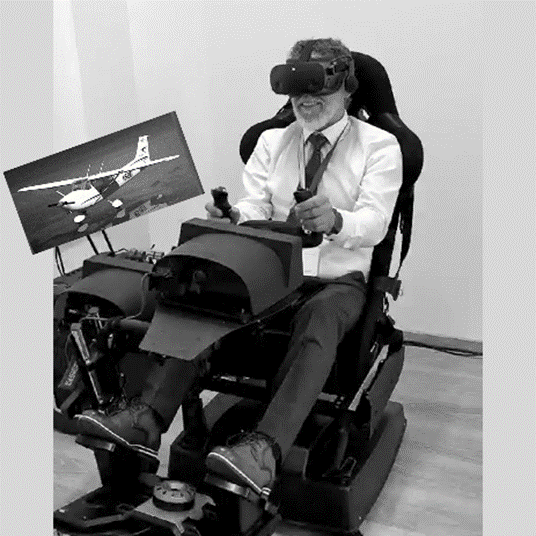
\includegraphics[width=1.0\textwidth]{images/Abbildung 1.png}
    \caption{\label{fig:Abbildung 1}Beispiel für VR-Flugsimulator (Full-motion)\protect
    }
\end{figure}
Dabei ist ein Vorteil des VR-Trainings die Fähigkeit des Simulators eine Welt sehr ähnlich unserer Welt zu replizieren, dadurch können die erlernenden Piloten/Pilotinnen trainieren ohne Schäden und Risiken einzugehen. Jedoch muss bei einem Flug Simulator auch darauf geachtet werden, dass der Simulator den erlernenden Piloten/Pilotinnen auch ein Gefühl des Fliegens vermittelt durch haptisches Feedback zum Beispiel, als Lösung kann ein full-motion Simulator dienen, da dieser auch Bewegung replizieren kann. Das Problem bei diesen full-motion Simulatoren ist, dass diese groß und kostenintensiv sind und deshalb meistens im Besitz von Fluggesellschaften, Leasingunternehmen oder unabhängigen Schulungsorganisationen sind, wodurch diese Simulatoren der Mehrheit der fliegenden Öffentlichkeit nicht zur Verfügung steht. In einer Studie von Ryan Guthridge und Virginia Clinton-Lisell wurden erlernenden Piloten/Pilotinnen in drei Gruppen aufgeteilt wurden, diese Gruppen haben dann jeweils eine andere Trainingsmethode benutzt, dies Methoden sein Computer-software-Training, VR-software-Training und einer Controll-Methode, die kein direktes Training machte sondern nur zuschaute. „In der Nachbefragung, der Studie, beschrieben die Teilnehmer die Vorteile der VR-Technologie als eine praktikable Methode zur Ausbildung von Studentenpiloten. Viele der Antworten waren konsistent und beinhalteten die "Fähigkeit, sich im Flugsimulator um das Flugzeug zu bewegen, indem die Flügel oder andere Objekte als Referenzpunkte verwendet werden". Einige Teilnehmer wiesen darauf hin, dass "VR für Studenten leichter verfügbar und kostengünstiger ist" im Vergleich zu teuren Flugausbildungsgeräten. Schließlich fügten einige Teilnehmer hinzu, dass "VR zu einem vernünftigen Preis für den Heimgebrauch verfügbar ist", was "bei der Vorbereitung auf Lektionen zu Hause vor dem Fliegen des echten Flugzeugs helfen kann". Mit der Weiterentwicklung der Technologie werden Flugschulorganisationen verstärkten Zugang zu kostengünstigen Simulator-alternativen haben. Diese Forschung liefert Beweise, die Pilotenleistungsvariablen sowie qualitative Akzeptanz- und Akzeptanzdaten vergleichen, um VR-Trainingsgeräte und PC-basierte Trainingsgeräte zu bewerten. \cite{guthridge2023evaluating}“ 
Insgesamt hat sich das VR-Training nachweislich positiv auf die Leistung von Studierenden während ihres Ausbildungsverlaufs ausgewirkt. Ganz angekommen ist die VR-Technologie noch nicht, aber wir sind uns ziemlich sicher, dass auch hier die VR-Technologie immer mehr und mehr benutzt werden wird.
Abbildung 1 \footnote{\url{https://legaltech.future-law.at/vr-flug-simulator-auf-der-ltk23/}}

\section{VR Training bei Bodenfahrzeugen}\label{sec:Bodenfahrzeugen}
VR Training bei Bodenfahrzeugen
Bei Autorennen werden VR-Simulatoren verwendet, die meist auch Lenkrad und Pedale mit beinhalten. Die meisten Rennfahrer benutzen diese um sich Rennstrecken einzuprägen und diese zu fahren. Jedoch ist das Training populärer bei Hobby-Rennfahrern als bei Professionellen Rennfahrern, da die Professionellen von ihrem Verein Trainingstrecken und Rennautos gestellt bekommen und dies natürlich ein besseres Training ist, da sie dabei ein zu eins das machen was sie trainieren. Bei dem VR Simulatoren fehlen meist bestimmte Einflüsse wie physische Störungen oder das Momentum, das auf den Körper übertragen wird beim Bremsen beziehungsweise Beschleunigen. Für Hobby-Sportler ist der VR-Simulator eine günstige und einfache Alternative auf berühmten Rennstrecken und sehr teuren Rennwägen zu fahren.
\\
\begin{figure}[!ht]
    \centering
    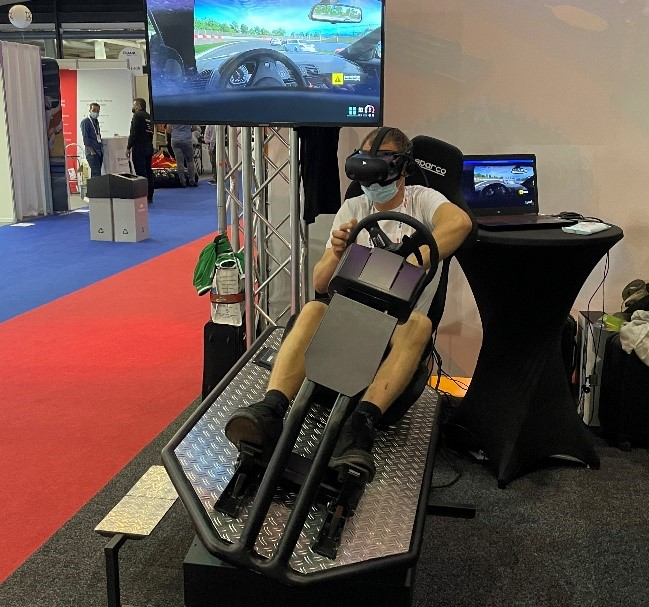
\includegraphics[width=1.0\textwidth]{images/Abbildung 2.jpg}
    \caption{\label{fig:Abbildung 2}Autorenn-Simulator (full-motion)\protect
    }
\end{figure}
Derzeitig wird jedoch auch an normalen Autofahr-Simulatoren (für Führerscheine) mit VR geforscht. Diese könnten bei Fahrlehrlingen die grade ihren Führerschein machen helfen, da wie auch bei den Rennsimulatoren kein echtes Auto und keine echte Straße benötigt wird. Das gibt die Vorteile in keine gefährlichen Situationen zu geraten, andere in keine gefährlichen Situationen zu bringen und die Kosten sind um einiges billiger. Dazu kann man mit verschiedenen Autos Trainieren. Am hilfreichsten ist der Autofahr-Simulator den Fahrlehrling zu trainieren was dieser in Stress- und Panik-Situationen macht ohne irgendein Risiko einzugehen \cite{ihemedu2017virtual}. Zusätzlich kann der Fahrlehrling Mut und Selbstsicherheit aufbauen währenddessen er im Simulator fährt und keine Fehler baut. Nachteile sind, dass man das Gefühl des Autofahrens nicht direkt übermittelt bekommt, dadurch können Sachen wie die Kupplung richtig benutzen und auch gefühlsvoll zu bremsen nicht wirklich durch den Simulator erlernt werden.
\\
\begin{figure}[!ht]
    \centering
    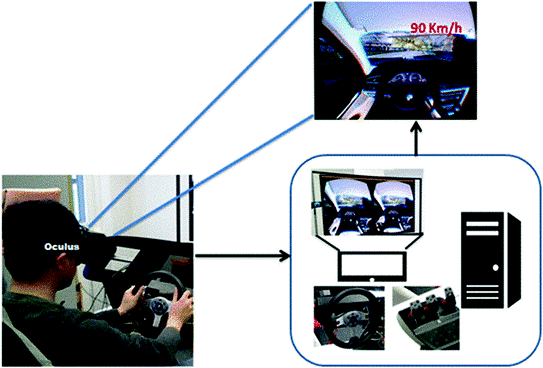
\includegraphics[width=1.0\textwidth]{images/Abbildung 3.png}
    \caption{\label{fig:Abbildung 3}Beispiel wie VR bei einer Fahrschule eingesetzt werden könnte\cite{ihemedu2017virtual}\protect
    }
\end{figure}
\\
Bei Bodenfahrzeugen ist VR-Training im Bereich der Rennautos weit entwickelt und wird von vielen benutzt, sogar von nicht-Sportlern, die einfach nur Spaß an einem VR-Spiel haben. Bei dem Trainieren von dem Auto fahren selbst ist die VR-Technologie noch kaum angekommen, aber es gibt positive Ausblicke das auch in diesem Teilbereich die VR-Technologie integriert wird und somit es leichter macht.

Abbildung 2 \footnote{\url{https://eveprocom.de/eventmodule/virtual-reality/full-motion-vr-racing-seat-pro-mieten/}}


\section{VR Training bei Automobilmanufaktur}\label{sec:Automobilmanufaktur}
Vr beim Auto manufaktur
Bei der Auto Manufaktur werden sogenannte VTS (Virtual-Trainings-Systeme verwendet. Bei einem dies VTS sieht der Benutzer eine Virtuelle Welt, in der er das das Auto sehen und verändern kann, dabei kann der Benutzer Schrauben, Motoren, Sitze und so weiter einbauen wie und wo er möchte.
\begin{figure}[!ht]
    \centering
    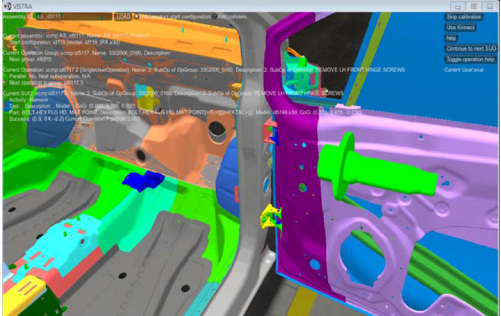
\includegraphics[width=1.0\textwidth]{images/Abbildung 4.png}
    \caption{\label{fig:Abbildung 4}Hier sieht man ein Beispiel dieser Virtuellen Welt durch das VTS VISTRA \cite{langley2016establishing}.\protect
    }
\end{figure}
Damit VR-Training bei der Autoherstellung akzeptiert werden kann, muss es als nützliche und effektive Trainingsmethode anerkannt werden. Dazu haben \cite{langley2016establishing} eine Studie gemacht bei der folgendes als Ergebnis herauskam: „Diese Arbeit hat begonnen, die Effektivität und Effizienz des ersten Prototyps des VTS (Virtual-training-system) mithilfe objektiver und subjektiver Maßnahmen zu etablieren. Allerdings hat diese Studie auch eine Reihe von Problemen identifiziert, die im nächsten Entwicklungs- und Verbesserungszyklus berücksichtigt werden. \cite{langley2016establishing} “.
\begin{figure}[!ht]
    \centering
    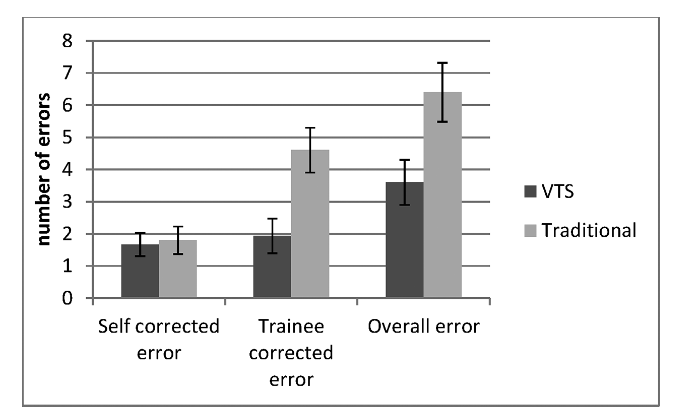
\includegraphics[width=1.0\textwidth]{images/Abbildung 5.png}
    \caption{\label{fig:Abbildung 5}In dieser Abbildung sieht man einen Vergleich von Ergebnissen der Studie von \cite{langley2016establishing}.\protect
    }
\end{figure}
Hier werden die selbst-behobenen Fehler, vom Trainer behobene Fehler und die Insgesamten Fehler von Lehrlingen, die zu einem das VTS benutzt haben und zum anderen die traditionale Variante benutzt haben, gezeigt. Hier sieht man das bei dem VTS insgesamt nur halb so viele Fehler passiert sind und daraus kann man schließen, dass durch den VTS-Fehler besser ausgeschlossen werden können\cite{langley2016establishing}.
Im Bereich der Automanufaktur ist die VR-Technologie noch kaum angekommen, aber da wo es angekommen ist bietet es Vorteile. Daraus lässt sich schließen, dass auch in diesem überraschenden Bereich, die VR-Technologie immer mehr und mehr benutzt werden wird.

\chapter{VR Training bei der Polizei}\label{sec:polizei}
In der modernen Welt der polizeilichen Ausbildung und Einsatzvorbereitung hat die virtuelle Realität (VR) eine bedeutende Rolle eingenommen. Die Integration von VR-Trainingstechnologien ermöglicht es  Polizeikräften realistische Szenarien zu simulieren und ihre Fähigkeiten in verschiedenen Bereichen zu verbessern. Diese Arbeit widmet sich der Analyse und Evaluation des Einsatzes von VR-Training bei der Polizei, wobei der Fokus auf folgenden Aspekten liegt: dem Umgang mit Stress und Amoksituationen (Abschnitt 3.1), der Forensik und Tatort-Untersuchung (Abschnitt 3.2) sowie der Missionen Planung und Kommunikation (Abschnitt 3.3).
\\
Die zunehmende Komplexität und Vielfalt der Herausforderungen, denen Polizeikräfte gegenüberstehen, erfordert innovative Trainingsmethoden, die über herkömmliche Ansätze hinausgehen. Die Anwendung von VR ermöglicht es den Polizeibehörden, realitätsnahe Szenarien zu schaffen, in denen die Einsatzkräfte ihre Reaktionsfähigkeiten in Stresssituationen trainieren können. Der Abschnitt 3.1 wird daher den Einfluss von VR-Training auf den Umgang mit Stress und Amoksituationen eingehend untersuchen, wobei die Wirksamkeit dieser Technologie bei der Steigerung der Belastbarkeit und Entscheidungsfähigkeit der Polizeibeamten analysiert wird.
\\
Im Abschnitt 3.2 wird der Schwerpunkt auf der forensischen und Tatort-Untersuchung liegen. VR-Technologien bieten ein immersives Umfeld, das es den Ermittlern ermöglicht, Tatorte zu rekonstruieren und forensische Analysen durchzuführen. Diese virtuellen Übungen können die Genauigkeit und Effizienz der Ermittlungen steigern. Die Arbeit wird die Integration von VR in diesen Prozessen eingehend beleuchten und die potenziellen Vorteile für die polizeiliche Arbeit herausstellen.
\\
Schließlich wird der Abschnitt 3.3 sich mit der Missionen Planung und Kommunikation befassen. Die Fähigkeit zur effektiven Planung und Koordination von Einsätzen ist entscheidend für den Erfolg polizeilicher Missionen. Hier wird untersucht, wie VR-Training die Zusammenarbeit und Kommunikation innerhalb von Polizeieinheiten verbessern kann, indem es realistische Simulationen von Einsatzszenarien bereitstellt. 

\section{Umgang mit Stress und Amoksituationen}\label{sec:polizei-SuA}
Ein großer Schwachpunkt des traditionellen Polizeitrainings ist der Umgang mit Stress und Amoksituationen. Durch normale Schießübungen und Probedurchläufe von Trainingseinheiten mit Dummys ist es unmöglich, eine realitätsgetreue Stresssituation nachzustellen. Wohin entgegen VR-Szenarien eine ähnlich hohe Stresslevel Höhe erreichen können, die sonst nur durch reale Konfliktsituationen erreicht wird. Das führt zur Folge, dass Polizisten echte Amoksituationen besser einschätzen und dementsprechend handeln können. Doch nicht nur die Einschätzung der Situation wird gefördert, sondern auch die Selbsteinschätzung. Durch die realitätsnahe Simulation werden charakteristische Eigenschaften der Polizisten offenbart. Dies dient dazu, falsche Herangehensweisen zu erkennen und zu verbessern, bevor diese in einer realen Situation passieren. Ein weiterer Vorteil des VR-Trainings ist die Wiederholungsmöglichkeit der Trainingslektion. Während bei den traditionellen Übungen Ressourcen wie Munition oder Trainingsdummys begrenzt und schwer wiederverwendbar sind, ist es mit Hilfe einer Virtual Reality Brille und einem Computerprogramm ganz einfach, ganze Trainingseinheiten zu Übungszwecken mehrfach zu wiederholen. \cite{kleygrewe2024virtual}
\\
Durch die Ersparnisse der Dauerkosten aufgrund von Ressourcenbeschaffung ist virtuelles Training trotz hoher Einmalkosten für Brillen und Programme günstiger als herkömmliche Trainingsmethoden. Außerdem werden Kosten gespart, indem veraltete Programme aktualisiert werden können, um dem heutigen Standard zu entsprechen. Deswegen können mehrere Generationen ausgebildet werden, ohne dass die Polizei ständig neue Ressourcen und Materialien zur Verfügung zu stellen muss. \cite{heltne2023cost}

\section{Forensik und Tatort-Untersuchung}\label{sec:polizei-FuT}
In der Tatort-Untersuchung ist die VR-Technologie eine immer häufiger auftauchende Alternative. Mit Hilfe einer vorgefertigten 3D-Welt werden Auszubildende in einen virtuellen Tatort versetzt, in dem sie sich frei-bewegen können, dort das Suchen von Spuren und das Bilden von Zusammenhängen zu lernen. Bewegen kann man sich in diesem Raum mit Hilfe von Sensoren, die den Körper tracken, oder durch Benutzung des Controllers. Diese Lernmethode beweist sich als besonders effektiv, da die meisten jungen Erwachsenen heutzutage bereits Erfahrung mit Videospielen haben. Sie empfinden die Übung weniger als Arbeit, da der spielerische Faktor überwiegt. Dieses Spiel ermöglicht es, schneller und einfacher zu lernen, währenddessen Kosten eingespart werden. Der einzige Makel der Anwendung ist die Bewegungskrankheit, die einem ein Übelkeitsgefühl geben kann, da der Körper Unstimmigkeiten zwischen visuell wahrgenommener Bewegung und dem Bewegungssinn aufweist. \cite{mayne2020virtual}
\\
Eine weitere Methode den Auszubildenden die Forensik näherzubringen, ist es, einen Tatort mit einer 360° Kamera einzuscannen und anschließend als Lernübung bereitzustellen. Anders als bei der vorherigen Methode kann hier jeder Schüler ganz einfach mit seinem Smartphone über einen QR-Code den Tatort analysieren. Das hat den Vorteil, dass das Lernen nicht standortabhängig ist und man auch in z.B. der Corona Zeit sein Wissen erweitern kann. \cite{kader2020building}

\section{Missionen Planung und Kommunikation}\label{sec:polizei-PuK}
Gute Kommunikation mit den Arbeitskollegen als auch mit Zivilpersonen ist eine Grundvoraussetzung für einen anerkannten Polizisten. Was früher ausschließlich durch Rollenspiele mit anderen Kollegen machbar war, ist heute mithilfe von auf virtuellen Szenarien basierenden Programmen erlernbar. Um hitzige Situationen durch Kommunikation zu entschärfen, werden Polizisten mit Hilfe einer VR-Brille in stressreiche und emotionale Situationen befördert. Das hat zum Vorteil, realitätsnahe Situationen einzustudieren, um bei einem echten Einsatz eigene, durch Stress ausgelöste Fehler zu minimieren. Außerdem erwies sich das Rollenspiel von Person zu Person als makelhaft, da es den Polizisten schwer fiel, den Partner als Rollenspiel Person anzuerkennen, weswegen es oft nötig war, professionelle Schauspieler zu engagieren. Um das empathische Denken weiter zu fördern, müssen Beamte in den VR-Simulationen oftmals auch die Rolle der Zivilperson einnehmen. \cite{kohl2023empathy}
\\
Während die Virtuelle Realität dabei hilft Kommunikation und Empathie zu Zivilpersonen zu erlernen, ist sie außerdem bei der Planung einer Mission und dementsprechend für die Kommunikation der Polizisten untereinander nützlich. 3D Modelle können mit Hilfe der erweiterten Realität (AR), durch geographische Informationen eine Abbildung des realen Einsatzgebietes darstellen. Diese können wiederum durch die VR-Technologie einstudiert und als Trainingseinheit verwendet werden, um das Fehlerrisiko auf ein Minimum zu beschränken.\cite{amorim2013augmented}

\section{Fazit}\label{sec:polizei-Fazit}
Die Benutzung der VR-Technologie bringt viele Vorteile mit sich. Sie bietet angehenden und ausgebildeten Polizisten die Chance sich weiterzuentwickeln und in Stresssituationen sich selbst als auch die aktuelle Situation besser einzuschätzen. Es wird ihnen leichter gemacht sich auf Amoksituationen durch VR-Trainingseinheiten vorzubereiten und ein besseres Verständnis zu bekommen was ihre Aufgaben und Vorgehensweisen sind. Hohe Einmalkosten, die durch die Ausstattung der VR-Brillen und Programme aufkommen sind im Gegensatz zu den Dauerkosten des traditionellen Trainings geringer. Durch 360° Scans und virtuell nachgestellte Tatorte fällt es der Forensik leichter, sich weiterzubilden und das teilweise, ohne das Haus verlassen zu müssen. Die Kommunikation wird beim VR-Training nicht vernachlässigt, da stressreiche Situationen nachgespielt und geübt werden können, ohne dass professionelle Schauspieler benötigt werden. Ebenfalls ist die Missionen Planung durch 3D Modelle, die mithilfe erweiterter Realität dargestellt und somit analysiert und studiert werden können, eine wesentliche Erleichterung.
\\
Abschließend kann man sagen, dass das Training in der Virtuellen Realität viele positive Aspekte mit sich bringt und nur wenig bis keine Kritikpunkte aufkommen. Deshalb kann man sich auf die Zukunft Freuen da sich diese Lernmethode immer weiterentwickelt und angewendet wird.

\chapter{VR Training in der Medizin}\label{sec:medizin}
VR-Training in der Medizin spielt eine große Rolle, da in der Medizin viel praktisch gearbeitet wird. Extremfälle und Operationen sind schwer zu testen und der Mangel an Übung kann zu fatalen Folgen führen. Durch das VR-Training wird dieses Problem gelöst und meist schwierige Operationen können somit gelehrt und geübt werden.


\section{Training bei Operationen}\label{sec:Operationen}
\input{kapitel/medizin/operation.tex}
\section{Training bei Ängsten und Phobien}\label{sec:ÄuP}
\input{kapitel/medizin/ÄuP.tex}
\section{Training für Reha}\label{sec:Reha}

Bei diesem Training werden Patienten vor allem bei Lähmungen verschiedene Aufgaben in einer Simulation gegeben und diese schrittweise erfüllt. Die Patienten bekommen eine Extralerneinheit zusätzlich zum eigentlichen Rehabilitationsprogramm\\

Idee\\
-Reha ist anstrengend und meist ist kaum Fortschritt spürbar 
durch ein VR-Training ist Fortschritt messbar und somit auch sichtbarer\\
-soll motivieren durch Extraprogramm\\
-Durch Spiegelung soll der Patient langsam Kontrolle über eigenen Körper wiedererlangen\\

Fazit\\
Ein VR-Training für Rehabilitation erweist sich besonders als hilfreich, da Patienten ihren eigenen Fortschritt erkennen können. Der eigene Fortschritt könnte diese dann motivieren und positive Effekt auslösen was zu einer schnelleren Genesung führen könnte. Es sollte aber nicht dass Programm ersetzen sondern es jeglich ergänzen






%\subsection{Unterkapitel}\label{sec:basics-subsection}
%\lipsum[1]


\chapter{Bilder, Tabellen und Listings}\label{sec:BilderTabellenListings}
\section{Bilder}
\subsection{Einfaches Bild volle Textbreite}\label{sec:images-textwidth}

\begin{figure}[!ht]
    \centering
    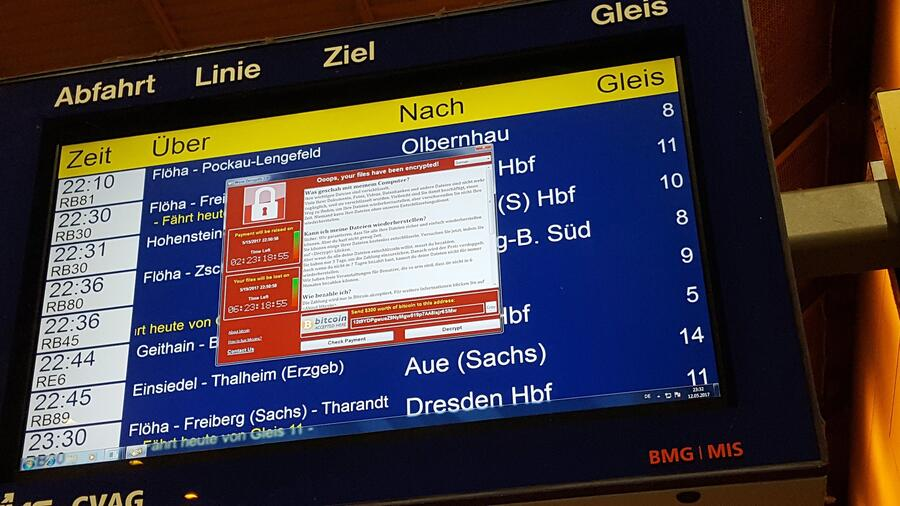
\includegraphics[width=1.0\textwidth]{images/example}
    \caption{\label{fig:example}Beispielbild\protect
    }
\end{figure}

In der Abbildung~\ref{fig:example} ist ein Beispielbild zu sehen.
Bilder werden mit \lstinline|\begin{figure}| eingeleitet.
Mit \lstinline|\includegraphics[width=1.0\textwidth]{Pfad/zum/Bild}| wird 
das Bild hinzugefügt, wobei das Bild durch die Zahl skaliert werden kann.
Das Pfad/zum/Bild ist mit dem relationalen Pfad zum Bild vom Projektordner aus zu ersetzen. 


\subsection{Mehrere Bilder nebeneinander}\label{sec:images-multiple}
\begin{figure}[!htb]
    \centering
    \hyperref[fig:big-example]{
    \minipage{0.46\textwidth}
        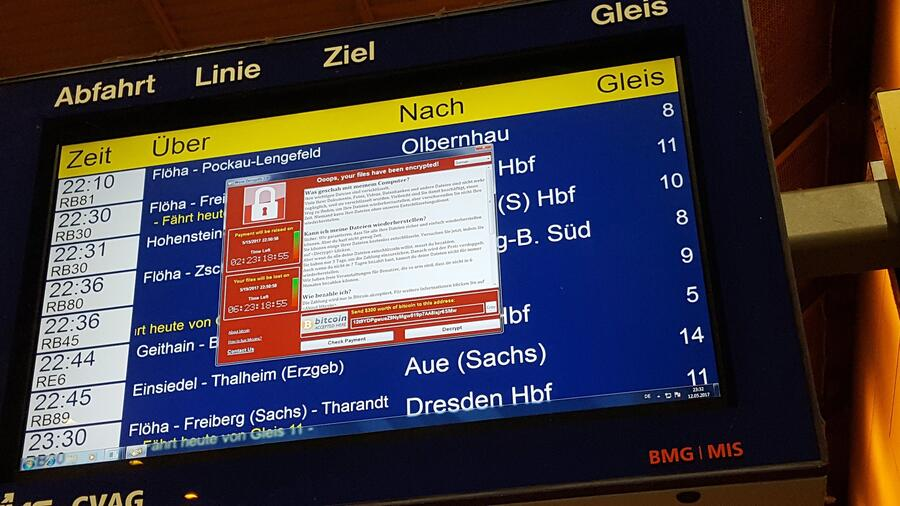
\includegraphics[width=\linewidth]{images/example}
        \caption{\label{fig:example-a}Beispielbild A}
    \endminipage\hfill
    }
    \hyperref[fig:big-example]{
    \minipage{0.46\textwidth}
        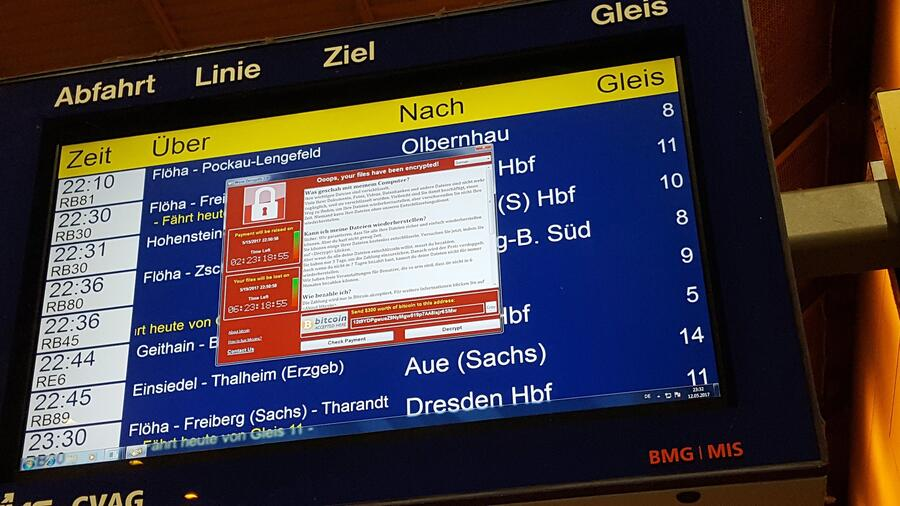
\includegraphics[width=\linewidth]{images/example}
        \caption{\label{fig:example-b}Beispielbild B}
    \endminipage\hfill
    }
    \hyperref[fig:big-example]{
    \minipage{0.46\textwidth}
        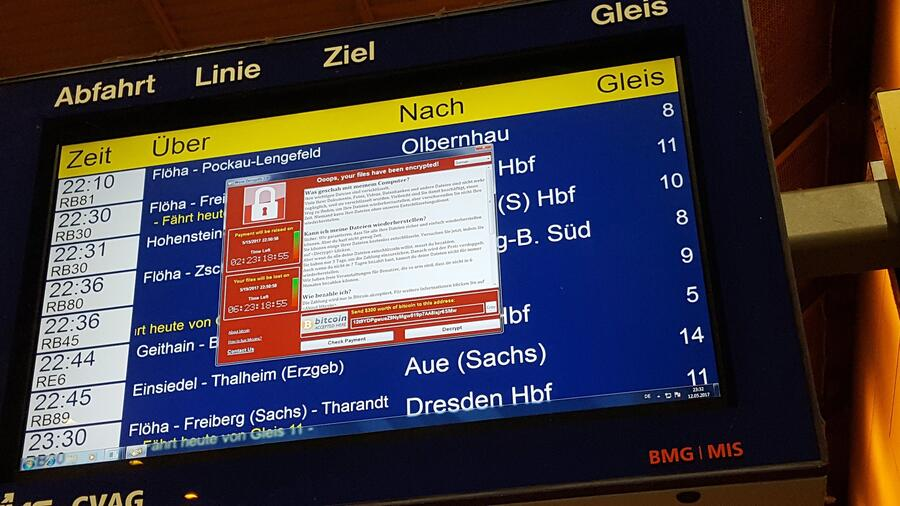
\includegraphics[width=\linewidth]{images/example}
        \caption{\label{fig:example-c}Beispielbild C}
    \endminipage\hfill
    }
    \hyperref[fig:big-example]{
    \minipage{0.46\textwidth}
        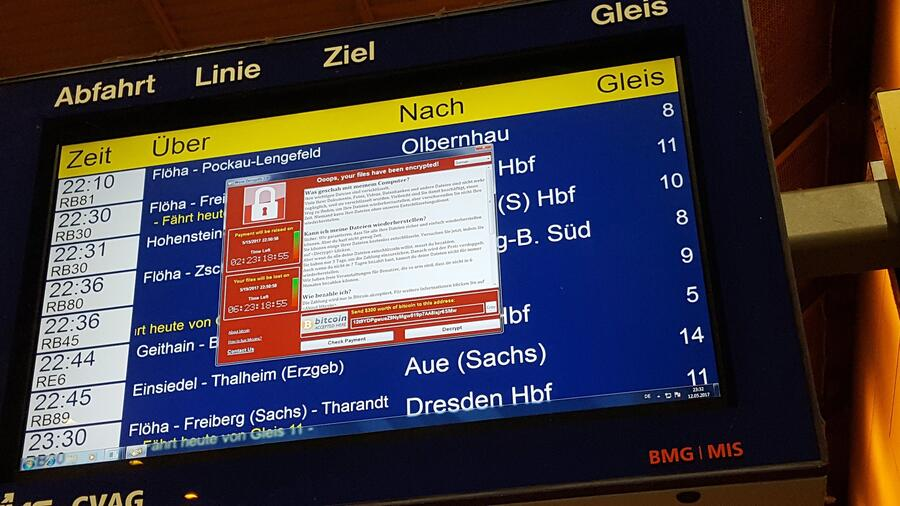
\includegraphics[width=\linewidth]{images/example}
        \caption{\label{fig:example-d}Beispielbild D}
    \endminipage\hfill
    }
    \caption{\label{fig:example-collection}Kollektion}
\end{figure}

In der \nameref{fig:example-collection} von Bildern in Abbildung~\ref{fig:example-collection}
ist die zusammenhängende Darstellung von Bildern gezeigt.
Die Bilder sind in den Anhang verlinkt. Wenn auf ein Bild geklickt wird, kann dieses 
in voller Größe im Anhang betrachtet werden.
Die Verlinkung ist in \path{attachments\bigpicture.tex} zu sehen.


\section{Tabellen}
\begin{table}[ht]
    \centering
    \begin{tabular}{ l c r }
        \toprule
                                & BIOS              & UEFI              \\
        \toprule
        \toprule
        Standardisiert          & Nein              & Ja                \\
        \midrule
        \midrule
        Aktualisierbar          & Nein              & Ja                \\
        \midrule
        \midrule
        Programmiersprache      & Assembler         & C                 \\
                                & schwer lesbar     & einfacher lesbar  \\
        \midrule
        \midrule
        Prozessormodus          & 16 Bit            & 32-64 Bit         \\
        Modulumsetzung          & Option-ROM        & Treiber           \\
        Parallele Ausführung    & Nein              & Ja                \\
        Geschwindigkeit         & Langsamer         & Schneller         \\
        \midrule
        \midrule
        \multicolumn{3}{l}{Verwendete Formatierung der Festplatten}\\
        \midrule
                                & MBR               & GPT               \\
                                & max 4 Partitionen & unlimitiert Partitionen\\
                                & max 2.1TB/HDD     & max 9.44ZB/HDD    \\
        \bottomrule
    \end{tabular}
    \caption{Vergleich von BIOS und UEFI}\label{tab:bios_uefi}
\end{table}

In Tabelle~\ref{tab:bios_uefi} ist ein Beispiel für eine Tabelle zu sehen.
Die Anzahl der Spalten wird nach \lstinline|\begin{tabular}| definiert.
Hier wird gleichzeitig auch die Textausrichtung mit c(=center),l(=left) oder r(=right) gesetzt werden. 
Die einzelnen Zellen der Tabelle werden mit \& voneinander getrennt und mit \lstinline|\\| beendet.
Mehrere Spalten können mit \lstinline|\multicolumn{x}{y}{Text}| verbunden werden,
wobei x die Anzahl der zusammengeführten Spalten und y die Textausrichtung (l, c oder r) ist.


\section{Listings}
\begin{lstlisting}[caption={HelloWorld Programm in Python},captionpos={b},label={lst:helloworld-python},language={Python}] 
    def main():
        print("Hello World\n");
        
    main()
\end{lstlisting}

Listings enthalten Quellcode von Programmen.
Das Beispiel in Listing~\ref{lst:helloworld-python} veranschaulicht das \nameref{lst:helloworld-python}.
Bei \lstinline|\begin{lstlisting}| sind in den eckigen Klammern folgende Eigenschaften definiert.
\begin{description}
    \item[caption] beinhaltet die Beschreibung des Listing
    \item[captionpos] positioniert die Beschreibung unter das Listing.
    \item[label] wird verwendet, um das Listing mit \lstinline|~\ref{lst:...}| im Text referenzieren zu können.
    \item[language] ist die Programmiersprache, die für das Markup verwendet wird.
\end{description}
Folgende Programmiersprachen sind im \lstinline|language|-Feld der Listings möglich.\\
ABAP2,4, ACSL, Ada4, Algol4, Ant, Assembler2,4, Awk4, bash, Basic2,4, C\#5, C++4, C4, Caml4, Clean, 
Cobol4, Comal, csh, Delphi, Eiffel, Elan, erlang, Euphoria, Fortran4, GCL, Go (golang), Gnuplot, Haskell, 
HTML, IDL4, inform, Java4, JVMIS, ksh, Lisp4, Logo, Lua2, make4, Mathematica1,4, Matlab, Mercury, MetaPost, 
Miranda, Mizar, ML, Modelica3, Modula-2, MuPAD, NASTRAN, Oberon-2, Objective C5 , OCL4, Octave, Oz, Pascal4, 
Perl, PHP, PL/I, Plasm, POV, Prolog, Promela, Python, R, Reduce, Rexx, RSL, Ruby, S4, SAS, Scilab, sh, SHELXL, 
Simula4, SQL, tcl4, TeX4, VBScript, Verilog, VHDL4, VRML4, XML, XSLT\footnote{Website mit unterstützten Programmiersprachen für Listings}. 


\chapter{Fazit}\label{sec:summary}
\section{Zusammenfassung}
Hier kommt die Zusammenfassung Ihrer Arbeit. 
Was haben Sie gemacht, welche Ergebnisse haben Sie erzielt. 

\section{Weitere Arbeiten}
Welche neue Ideen haben sich ergeben? 
Was müsste weiter untersucht werden? 
Welche weiteren Bachelor- oder Masterarbeiten sind in dem Themenfeld nun interessant geworden? 

\backmatter

\chapter{Glossar und Akronyme}\label{sec:glossary}
Die Beschreibung des Begriffs \gls{acronym} wird im Glossar erklärt.
Hierfür wird in der Datei \path{appendix/glossary.tex} der entsprechende Eintrag hinzugefügt.
Mit dem \lstinline|\gls{glossar-referenz}| Befehl kann man die Begriffe im Text auf direkt in das Glossar verlinken.\\
\par
\glspl{acronym} selbst wie beispielsweise \gls{rz}, werden beim ersten mal ausgeschrieben.
Wird \gls{rz} ein zweites Mal verwendet, ist nur die Abkürzung im Text zu sehen.
\glspl{acronym} werden in der Datei \path{attachments/acronyms.tex} definiert und 
können zur Definition des \gls{acronym}s in das Glossar weiter verlinkt werden.


% Für die Akronyme, die Literatur und das Glossar wird der Zeilenabstand reduziert.
\singlespacing{}
% Hier werden die Akronyme und das Glossar in das Dokument geschrieben
\printnoidxglossary[type=\acronymtype,title={Abkürzungen\label{akronyme}}]
% Glossaa
\printnoidxglossary[title={Glossar}]

% Hier wird das Literaturverzeichnis in das Dokument geschrieben
% Das Literaturverzeichnis bekommt keine Kapitelnummer im Inhaltsverzeichnis und wird mit einem * versehen
\newpage
\addcontentsline{toc}{chapter}{Literatur}
\bibliographystyle{alpha}
\bibliography{references}

\newpage
% Anhang erstellen, da dieser ebenfalls keine Nummerierung bekommt,
% wird wieder der Asterix (*) nach \chapter verwendet.
\chapter{Anhang}\label{appendix}
\section{Zusätzliche Informationen}\label{att:bigpicture}
Im Anhang platzieren Sie weitere Informationen aus dem Kontext Ihrer Arbeit.
Wichtige Ergebnisse, die Sie erzielt haben, gehören allerdings nicht hierher.
\end{document}
